\afterpage{
\begin{figure}[H]
\centering
    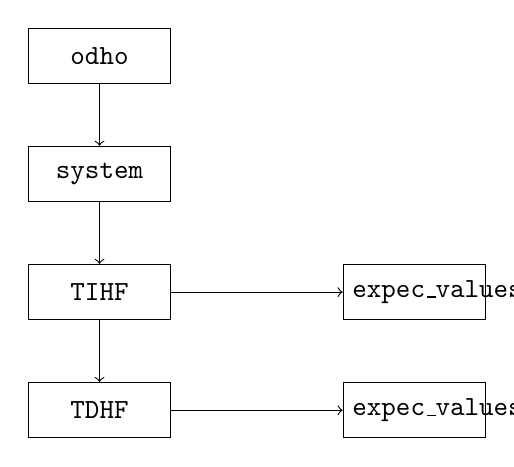
\begin{tikzpicture}
        %[draw, line width=0.3mm, text width=0.13\textwidth, minimum height=30pt, text centered]
        
        \node (odho) [draw, text width=0.13\textwidth, minimum height=20pt, text centered] at (4,0) {\bfseries \texttt{odho}};
        \node (system) [draw, text width=0.13\textwidth, minimum height=20pt, text centered] at (4, -1.5) {\texttt{system}};
        \node (TIHF) [draw, text width=0.13\textwidth, minimum height=20pt, text centered] at (4, -3) { \texttt{TIHF}};
        \node (TDHF) [draw, text width=0.13\textwidth, minimum height=20pt, text centered] at (4, -4.5) { \texttt{TDHF}};
        
        \node (expvalueTIHF) [draw, text width=0.13\textwidth, minimum height=20pt, text centered] at (8, -3) {\texttt{expec\_values}};
        \node (expvalueTDHF) [draw, text width=0.13\textwidth, minimum height=20pt, text centered] at (8, -4.5) { \texttt{expec\_values}};
        
        \draw [->, to path={-| (\tikztotarget)}] (odho.south) -- (system.north);
        \draw [->, to path={-| (\tikztotarget)}] (system.south) -- (TIHF.north);
        \draw [->, to path={-| (\tikztotarget)}] (TIHF.south) -- (TDHF.north);
        \draw [->, to path={-| (\tikztotarget)}] (TIHF.east) -- (expvalueTIHF.west);
        \draw [->, to path={-| (\tikztotarget)}] (TDHF.east) -- (expvalueTDHF.west);
        
    \end{tikzpicture}
    \caption{Diagram describing the workflow behind the implemented code. The \texttt{odho} object is employed for the costruction of the \texttt{system}, which then provides the instruments for the time-dependent and time-independent solvers.}
    \label{diag:code_structure}
\end{figure}
}
We chose Python as a programming language for this project. 
Our program is developed as a Jupyter Notebook, while all the functions and the information on the considered systems are enclosed in a class defined on a separated Python file.
Employing a class for the considered problem allows us to escape from the need of passing many parameters to the implemented functions, using instead the attributes of the class as global variables.

The creator implemented inside the class builds the system, which then can be manipulated and time-evolved by mean of functions defined in the same framework.
The entire program is based on the functions provided in the \texttt{quantum-system} library \cite{gitOyvind}.
This uses finite-difference methods to solve a one-body Hamiltonian $h$ for an arbitrary potential of the form $V(r_i)$, which for our case was chosen to be the harmonic one with frequency $\Omega$. Considering the general representation of the spin, when the creator is called an \texttt{odho} object is built: it contains the first $l$ eigenstates evaluated on a mesh and the corresponding bra-kets appearing in Eq.s \ref{eq:h_elements}, \ref{eq:x_elements} and \ref{eq:u_elements} evaluated between all the possible combinations of the eigenstates. The so-built basis set is then used for the construction of the actual \texttt{system}, namely including the general spin treatment in the problem. The number of basis functions is doubled, with even indexes referring to the spin-up components and odd indexes to the spin-down counterparts. The dimensions of all the matrixes previously mentioned are doubled too. 

After the creation of the system, functions implemented within the class allow to solve the Hartree-Fock equations both with and without the laser source. Other functions take as input the so-obtained coefficients matrix for the ground state to evaluate the expected values presented in the previous sections. Alternatively they can be exploited to proceed with the time evolution of the system and perform the various tasks required for the project. \\

A subclass was implemented for the restricted representation of the spin: here the same reasoning described above applies too, but the attribute \texttt{system} actually coincides with the mentioned \texttt{odho}, since, as seen also in Section \ref{sec:restricted_HF}, the problem can be solved without doubling the number of basis functions to allow for spin mixing.


\begin{minted}[frame=lines, bgcolor=lemonchiffon]{python}
import needed_packages 

class GHF():
    def __init__():
        odho = ODQD([args])
        self.system = 
            GeneralOrbitalSystem([args])
    
    # time-independent HF solver
    def solve_TIHF([args])
    
    # time-dependent HF solver
    def solve_TDHF([args])
    
    # other functions
    def functions()

class RHF(GHF):
    def __init__():
        self.system = ODQD([args])
    
    # adapts some functions from GHF to the
    # RHF case
    def functions_changed()
    
\end{minted}

 
